\documentclass{article}
\usepackage[a4paper]{geometry}
\usepackage{graphicx}
\usepackage{hyperref}
\usepackage{float}
\usepackage{tikz}
\usepackage{amsmath}
\usepackage{graphicx}
\usepackage[affil-it]{authblk}\hypersetup{
    colorlinks,
    citecolor=black,
    filecolor=black,
    linkcolor=black,
    urlcolor=black
}
\usepackage{apacite}
\usepackage[authoryear]{natbib}

\setlength{\parindent}{0pt}
\setlength{\parskip}{1em}

\title{Evolutionary Models with a Large Number of Genes}
\author{
    Mher Saribekyan, Suren Hakobyan, Davit Badalyan\\
    Instructor: Varazdat Stepanyan 
}
\affil{American University of Armenia}
\date{November 2024}
\begin{document}
\maketitle
\newpage
\tableofcontents
\newpage

\section{Introduction}
Have you ever asked yourself how humanity has reached its current state of being? Have you ever wondered how some species (including humans) survived throughout centuries of changing environment, while others went extinct? The answer to these and many other questions lie in the broad study of evolution. 

According to Cambridge Dictionary, evolution is defined as \textit{"the way in which living things change and develop over millions of years."} Living things inevitably change over time due to multiple reasons. For example, a long-term food shortage caused by the change in the environment can force a given species to eat less, which over time will affect the next generations of the same species. The new generations might become more and more resistant to starvation and require less nutrition to survive. During this transition, many representatives of the species might die, and in some cases the species might fail to adapt and go extinct. However, if it \textbf{evolves} successfully, then the species will continue it's existence in the new environment, which might once again change in the future. 

A more scientific definition to the term evolution was given by Douglas Futuyma in his popular textbook.

\begin{quotation}
    [biological evolution] is change in the properties of groups of organisms over the course of generations…it embraces everything from slight changes in the proportions of different forms of a gene within a population to the alterations that led from the earliest organism to dinosaurs, bees, oaks, and humans.
\end{quotation}

Evolution can occur by different means, such as natural selection, genetic drift, mutation, migration and so on. This report will simulate the process of species evolving over time by adapting to their environment through mutations and natural selection. It will explore scenarios with different starting conditions, where diverse creatures with unique genes inhabit varying environments. The study will examine how these genes mutate over time and determine which mutations dominate in each specific setting.
\newpage

\section{Glossary}

Let one first establish some notions which are being discussed throughout this report.

\subsection{Natural Selection}

Elena Racevska defined natural selection as follows.

\begin{quotation}
    Natural selection is a process by which organisms that are better adapted to specific pressures of their environment tend to survive longer and produce more offspring, thus ensuring the preservation and multiplication of those favorable traits through generations, at the expense of the less advantageous ones.
\end{quotation}

If there were no limitations on any species, then it would boundlessly grow. The nature is preventing this by imposing various limitations and creating an environment where species need to survive by adapting to the realities around them. Such limitations may include food limitations, disadvantageous climate conditions, diseases, natural disasters, rival species and so on. In this way, the nature "selects" those species which will be able to reproduce and hence create an evolutionary change. The article published at Stanford University makes in interesting analogy. 

\begin{quotation}
    Much like breeders choose which of their animals will reproduce and thereby create the various breeds of domesticated dogs, pigeons, and cattle, nature effectively “selects” which animals will breed and creates evolutionary change just as breeders do.
\end{quotation}

\subsection{Mutation}

A mutation is a change in a genetic sequence. In biology, it is usually discussed as a negative alteration of a creature's genetic code, which causes various genetic diseases. In the scope of this paper, a mutation is the change in the genome of an offspring compared to genome of it's parent. That is, when a creature reproduces, the genes of it's off-springs might be slightly modified (also called somatic mutation). Some traits of the offspring might remain the same, others might change.

\subsection{Asexual Reproduction}

The species which is being simulated in this report reproduce asexually. The Journal of Evolutionary Biology put the definition of asexual reproduction in the following manner.

\begin{quotation}
    Asexual reproduction occurs when an individual produces new individuals that are genetically identical to the ancestor at all loci in the genome, except at those sites that have experienced somatic mutations.
\end{quotation}

In simpler terms, each representative of a species reproduce on its own and copies itself, with a chance that the offspring (copy) will have a slightly mutated, modified genome.

\section{Simulation Setting}

Let one first define the simulation setting. Each simulation is a collection of time steps. First, the environment and all of its components are being initialized, then the generated entities iterate through a predefined number of steps, and finally at the end the data is being collected and analyzed.

\subsection{Creature}

A creature is a single representative of the species one is observing. Each time step, a creature is looking around in search for food, goes towards the food if it sees any, and eats the food if the food is nearby. The creature can also decide to battle another creature if they are in the same location and eat them in case of victory. If in a favorable position, the creature will reproduce, creating an offspring.

Each creature has a genome, a position in the environment and an energy level. Let one discuss each of these separately.

\subsubsection{Genome}

The genome of a creature is what defines the characteristics (traits) of that creature. It resembles the DNA of the creature which is predefined by nature. The genome and it's change through generations is how evolution is observed, and it is the primary focus of this study.

The genome consists of 5 individual genes, each of which depicts a certain trait. Here are the general descriptions of the traits.

\begin{enumerate}
    \item \textbf{Speed} - determines the maximal distance that the creature can travel in a single time step.
    \item \textbf{Eyesight} - determines the area which is visible to the creature. It is mostly used to locate food and move towards it.
    \item \textbf{Aggression} - determines if the creature will engage in a fight or not. A higher aggression value means that the creature is more likely to start a battle, while a lower value means the creature is more likely to avoid contact and mind it's own business.
    \item \textbf{Strength} - determines the physical abilities of the creatures in case of a fight. A creature with a higher strength value is more likely to win the battle against a creature with a lower strength value.
    \item \textbf{Stamina} - determines the endurance of the creature, how long can the creature last without resources and at most how much energy it can store in itself. 
\end{enumerate}

\subsubsection{Position}

The position of a creature describes the location of the creature in a given environment. Position has different meanings depending on different environments. For example, the position of a creature on a plane is a coordinate pair $(x, y)$, on a line its a single number, in space its a coordinate triple $(x, y, z)$ and so on. For each environment, the position will be separately defined, which majorly affects on how creatures move, hence affecting the evolution.

\subsubsection{Energy}

The energy of a creature showcases the physical power left in the creature to continue surviving. A non-positive value for the energy means that the creature has no power left and hence dies. Each time step, every creature loses energy on moving and supporting their physical existence. Creatures gain energy by eating food or other creatures if they win in a battle. The energy is also used to reproduce, since a certain threshold of energy must be satisfied so that the creature is able to reproduce.

Each creature has maximal energy. The maximal energy a creature can have is determined by the stamina of the creature. If the creature has a higher stamina, then it has a higher capacity to store energy, while a lower stamina will result in a lower maximal energy.

\subsection{Reproduction and Mutations}

The species in question reproduce asexually. If a creature gains energy with a certain ratio of its maximal energy, it reproduces, gives 1 offspring, and loses a certain ratio of its energy because of it. It is the only way a creature can spawn in naturally in the simulation, except the initially generated creatures at the beginning of the simulation.

The offspring is spawned in an adjacent position and each gene is copied from its parent, with a certain probability for each gene to change by a value of 1.

\subsection{Memory optimization}
The creature is defined as an unsigned 32-bit integer, where the first 16 bits represent the genome, the next 12 bits represent its position cell and the last 4 bits represent the energy.

\subsection{Energy loss}

\[\text{energy loss}=\text{steps}+\left\lceil\frac{\text{eyesight}}{3}\right\rceil+\left\lfloor\frac{\text{aggression}}{5}\right\rfloor+\left\lfloor\sqrt{\text{strength}}\right\rfloor+\left\lfloor\frac{\text{stamina}}{7}+1\right\rfloor\]
\[\text{eyesight}\in\{0,1,...,7\}\]
\[\text{aggression}\in\{0,1,...,7\}\]
\[\text{strength}\in\{1,2,...,16\}\]
\[\text{stamina}\in\{-7,-6,...,8\}\]

All these values have an effect on how much energy the creature spends. Steps are the number of steps. We have no energy loss from aggression, up until the value of 5.

\begin{table}[H]
\begin{center}
    \begin{tabular}{|p{0.11\linewidth} |p{0.08\linewidth}|p{0.7\linewidth}|}
    \hline
    Gene & Bits & Description  \\\hline
    Speed & 2 & Takes values between 1 and 4, showing the Manhattan distance the creature can walk in a single timestep.\\\hline
    Eyesight & 3 & Takes values between 0 and 7, showing the Manhattan distance the creature can see.\\\hline
    Aggression & 3 & Takes values between 0 to 7, mapped to 0\% - 100\%, showing the probability of the creature attacking another creature in the same cell. \\\hline
    Strength & 4 & Takes values between 1 and 16, which determines the winner in a fight \\\hline
    Stamina & 4 & Takes values between -7 and 8, which is added to the base energy level, when generating the creature\\\hline
\end{tabular}
\caption{Creature characteristics and their descriptions}
\end{center}
\end{table}
\begin{figure}[!h]
\begin{center}
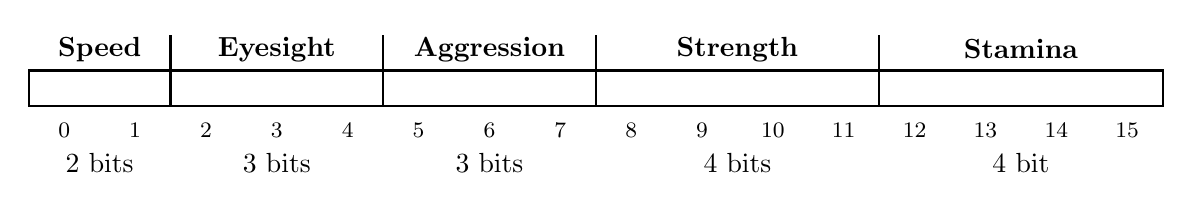
\begin{tikzpicture}[scale=0.9]
    % Draw the main rectangle for the 32 bits
    \draw[thick] (-0.5, 0) rectangle (15.5, 0.5);
    
    % Draw internal divisions for fields
    \foreach \x in {1.5, 4.5, 7.5, 11.5} {
        \draw[thick] (\x, 0) -- (\x, 1);
    }

    % Label the fields
    \node at (0.5, 0.8) {\textbf{Speed}};
    \node at (3, 0.8) {\textbf{Eyesight}};
    \node at (6, 0.8) {\textbf{Aggression}};
    \node at (9.5, 0.8) {\textbf{Strength}};
    \node at (13.5, 0.8) {\textbf{Stamina}};
    
    % Add labels for the bit positions (0-31)
    \foreach \x in {0, 1, ..., 15} {
        \node[anchor=north] at (\x, -0.1) {\footnotesize \x};
    }

    % Field descriptions under each field
    \node at (0.5, -0.8) {2 bits};
    \node at (3, -0.8) {3 bits};
    \node at (6, -0.8) {3 bits};
    \node at (9.5, -0.8) {4 bits};
    \node at (13.5, -0.8) {4 bit};
\end{tikzpicture}
\caption{Gene storage}
\end{center}
\end{figure}
\begin{figure}[!h]
\begin{center}
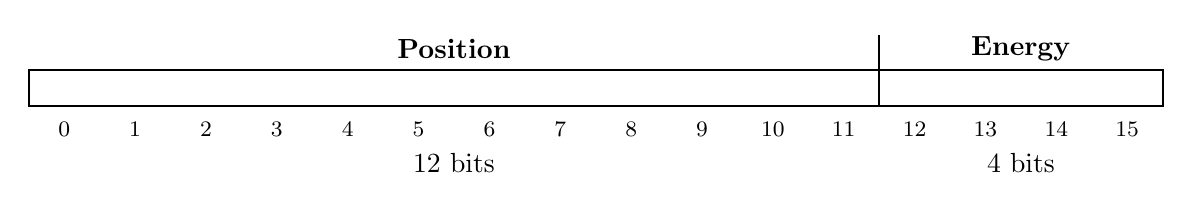
\begin{tikzpicture}[scale=0.9]
    % Draw the main rectangle for the 32 bits
    \draw[thick] (-0.5, 0) rectangle (15.5, 0.5);
    
    % Label the fields
    \node at (5.5, 0.8) {\textbf{Position}};
    \draw[thick] (11.5, 0) -- (11.5, 1);
    \node at (13.5, 0.8) {\textbf{Energy}};
    
    % Add labels for the bit positions (0-31)
    \foreach \x in {0, 1, ..., 15} {
        \node[anchor=north] at (\x, -0.1) {\footnotesize \x};
    }

    % Field descriptions under each field
    \node at (5.5, -0.8) {12 bits};
    \node at (13.5, -0.8) {4 bits};
\end{tikzpicture}
\caption{Position storage}
\end{center}
\end{figure}
The creatures are stored in a list and are iterated over in every timestep.
\section{Results}
The following constants were chosen for our simulations:
\begin{table}[H]
    \begin{center}
        \begin{tabular}{|p{0.24\linewidth} |p{0.08\linewidth}|p{0.55\linewidth}|}
        \hline
        Constant & Value & Notes  \\\hline
        Grid size & \(64\) & \(2^6\times 2^6\) grid\\\hline        
        Food cap & 0.05 & 5\% of the grid\\\hline
        Init creatures & 0.01 & We start with 1\% of the grid being creatures\\\hline
        Steps & 10000 & Number of timesteps\\\hline
        Base energy & 8 & Base energy\\\hline
        Energy from food & 5 & Energy gained from consuming food\\\hline
        Energy from creature & 8 & Energy gained from consuming another creature\\\hline
        Energy ratio to reproduce & 0.9 & When energy level reaches 90\% of the creatures max energy, it reproduces\\\hline
        Energy ratio for reproduce & 0.2 & 20\% of energy is consumed for reproduction\\\hline
        Number of children & 1 & Each reproduction only produces a single offspring\\\hline
        Mutation probability & 0.01 & There is a 1\% change for each gene to mutate during reproduction\\\hline
    \end{tabular}
    \caption{Creature characteristics and their descriptions}
    \end{center}
    \end{table}
\begin{center}
    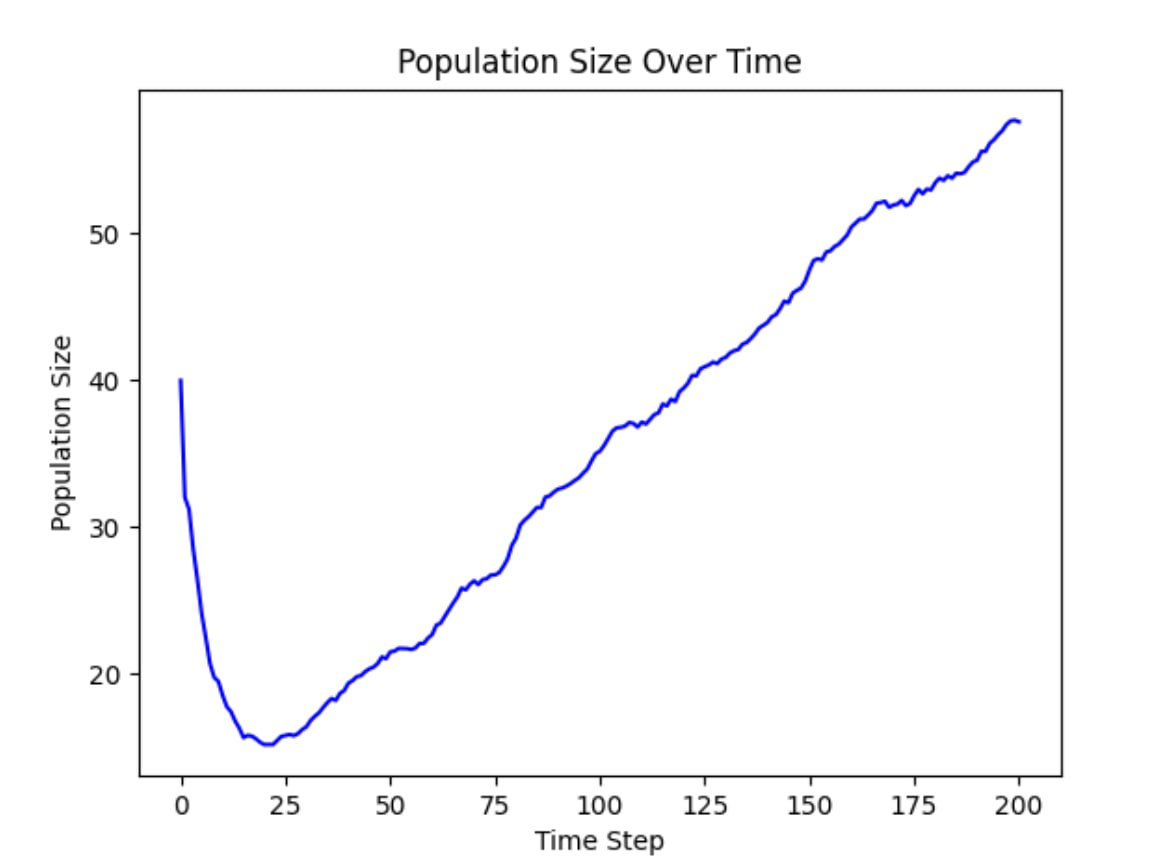
\includegraphics[scale=0.2]{images/image1.jpg}
\end{center}
\begin{center}
    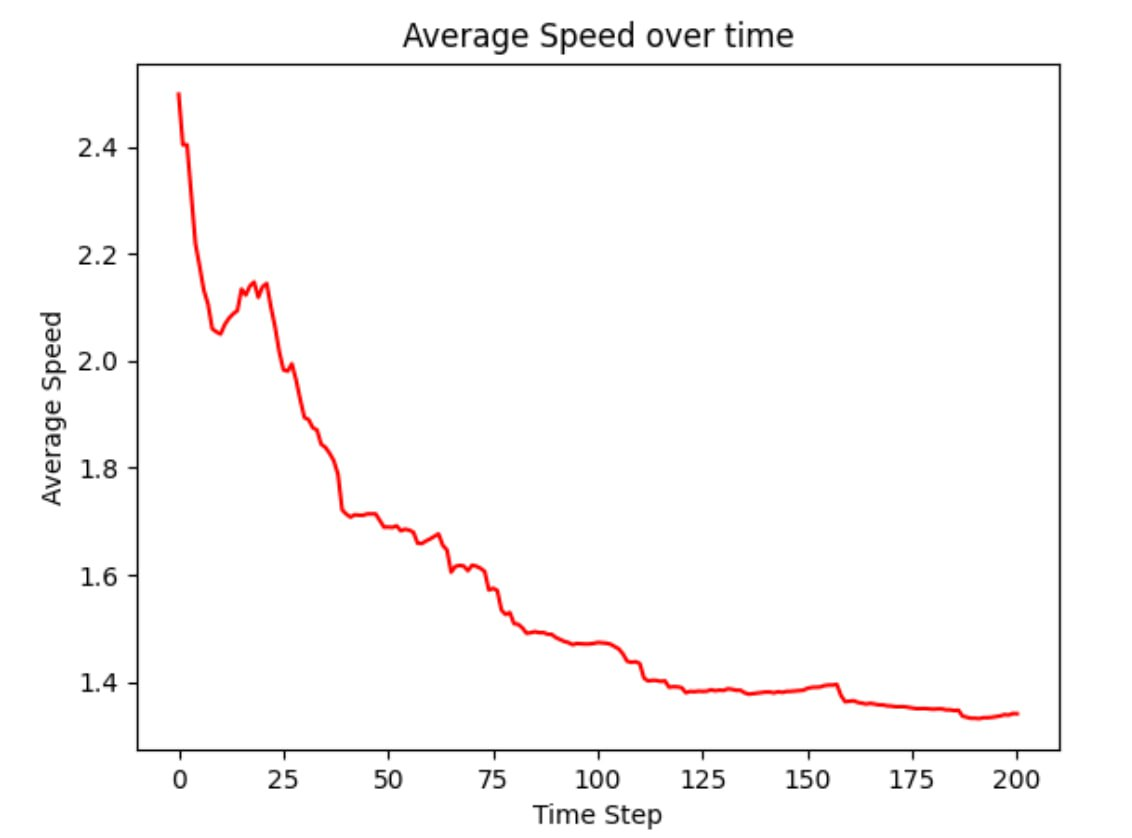
\includegraphics[scale=0.2]{images/image2.jpg}
\end{center}
Code is availabe at \href{https://github.com/suren2003ah7/EvolutionaryModel}{https://github.com/suren2003ah7/EvolutionaryModel}.
\section{Discussion}
We have simulated the model with several cases, however we may try on more complex cases.

\begin{enumerate}
    \item Random genes. Try many random genes for creatures and see if we reach equilibrium of one gene.
    \item Strong specific genes. Start with high values for specific genes and see if we reach equilibrium or not after mutaitons.
    \item Record the evolution of each gene by averaging that genes during each timestep.
\end{enumerate}
\nocite{*}
\bibliographystyle{apacite}
\bibliography{refs}
\end{document}